\chapter{Synthèse}

Dans cette version 2.1 du Mastermind vous trouverez des leds mais aussi des niveaux, cinq en tout (extrait du commentaire final du programme):
\begin{enumerate}
\item \emph{Beginner} : niveau débutant, "finger in the nose"
	\begin{itemize}
      \item Pas le droit à plusieurs fois la même lettre
      \item Les lettres possible sont de A à E
	\end{itemize}
    
\item \emph{Normal} : règles officielle du Mastermind
	\begin{itemize}
      \item Pas le droit à plusieurs fois la même lettre
      \item Les lettres possible sont de A à F
	\end{itemize}
    
\item \emph{Teacher} : règles demandées dans le sujet du projet
	\begin{itemize}
      \item Plusieurs même lettres possibles
      \item Les lettres possible sont de A à F
	\end{itemize}
    
\item \emph{Hard} : niveau difficile, "Good Luck !"
	\begin{itemize}
      \item Plusieurs même lettres possibles
      \item Les lettres possible sont de A à G
	\end{itemize}
    
\item \emph{42} : niveau solution 404 "Fuyez Pauvres Fous!"
	\begin{itemize}
      \item Plusieurs même lettres possibles
      \item Les lettres possible sont tout l'alphabet !!
	\end{itemize}
\end{enumerate}

\newpage
\section{Programme}
\underline{Code source du programme:}
\lstinputlisting{Sources/Mastermind.ino}

\newpage
\section{Quelques images de la version finale:}
\begin{figure}[h]
	\centering
		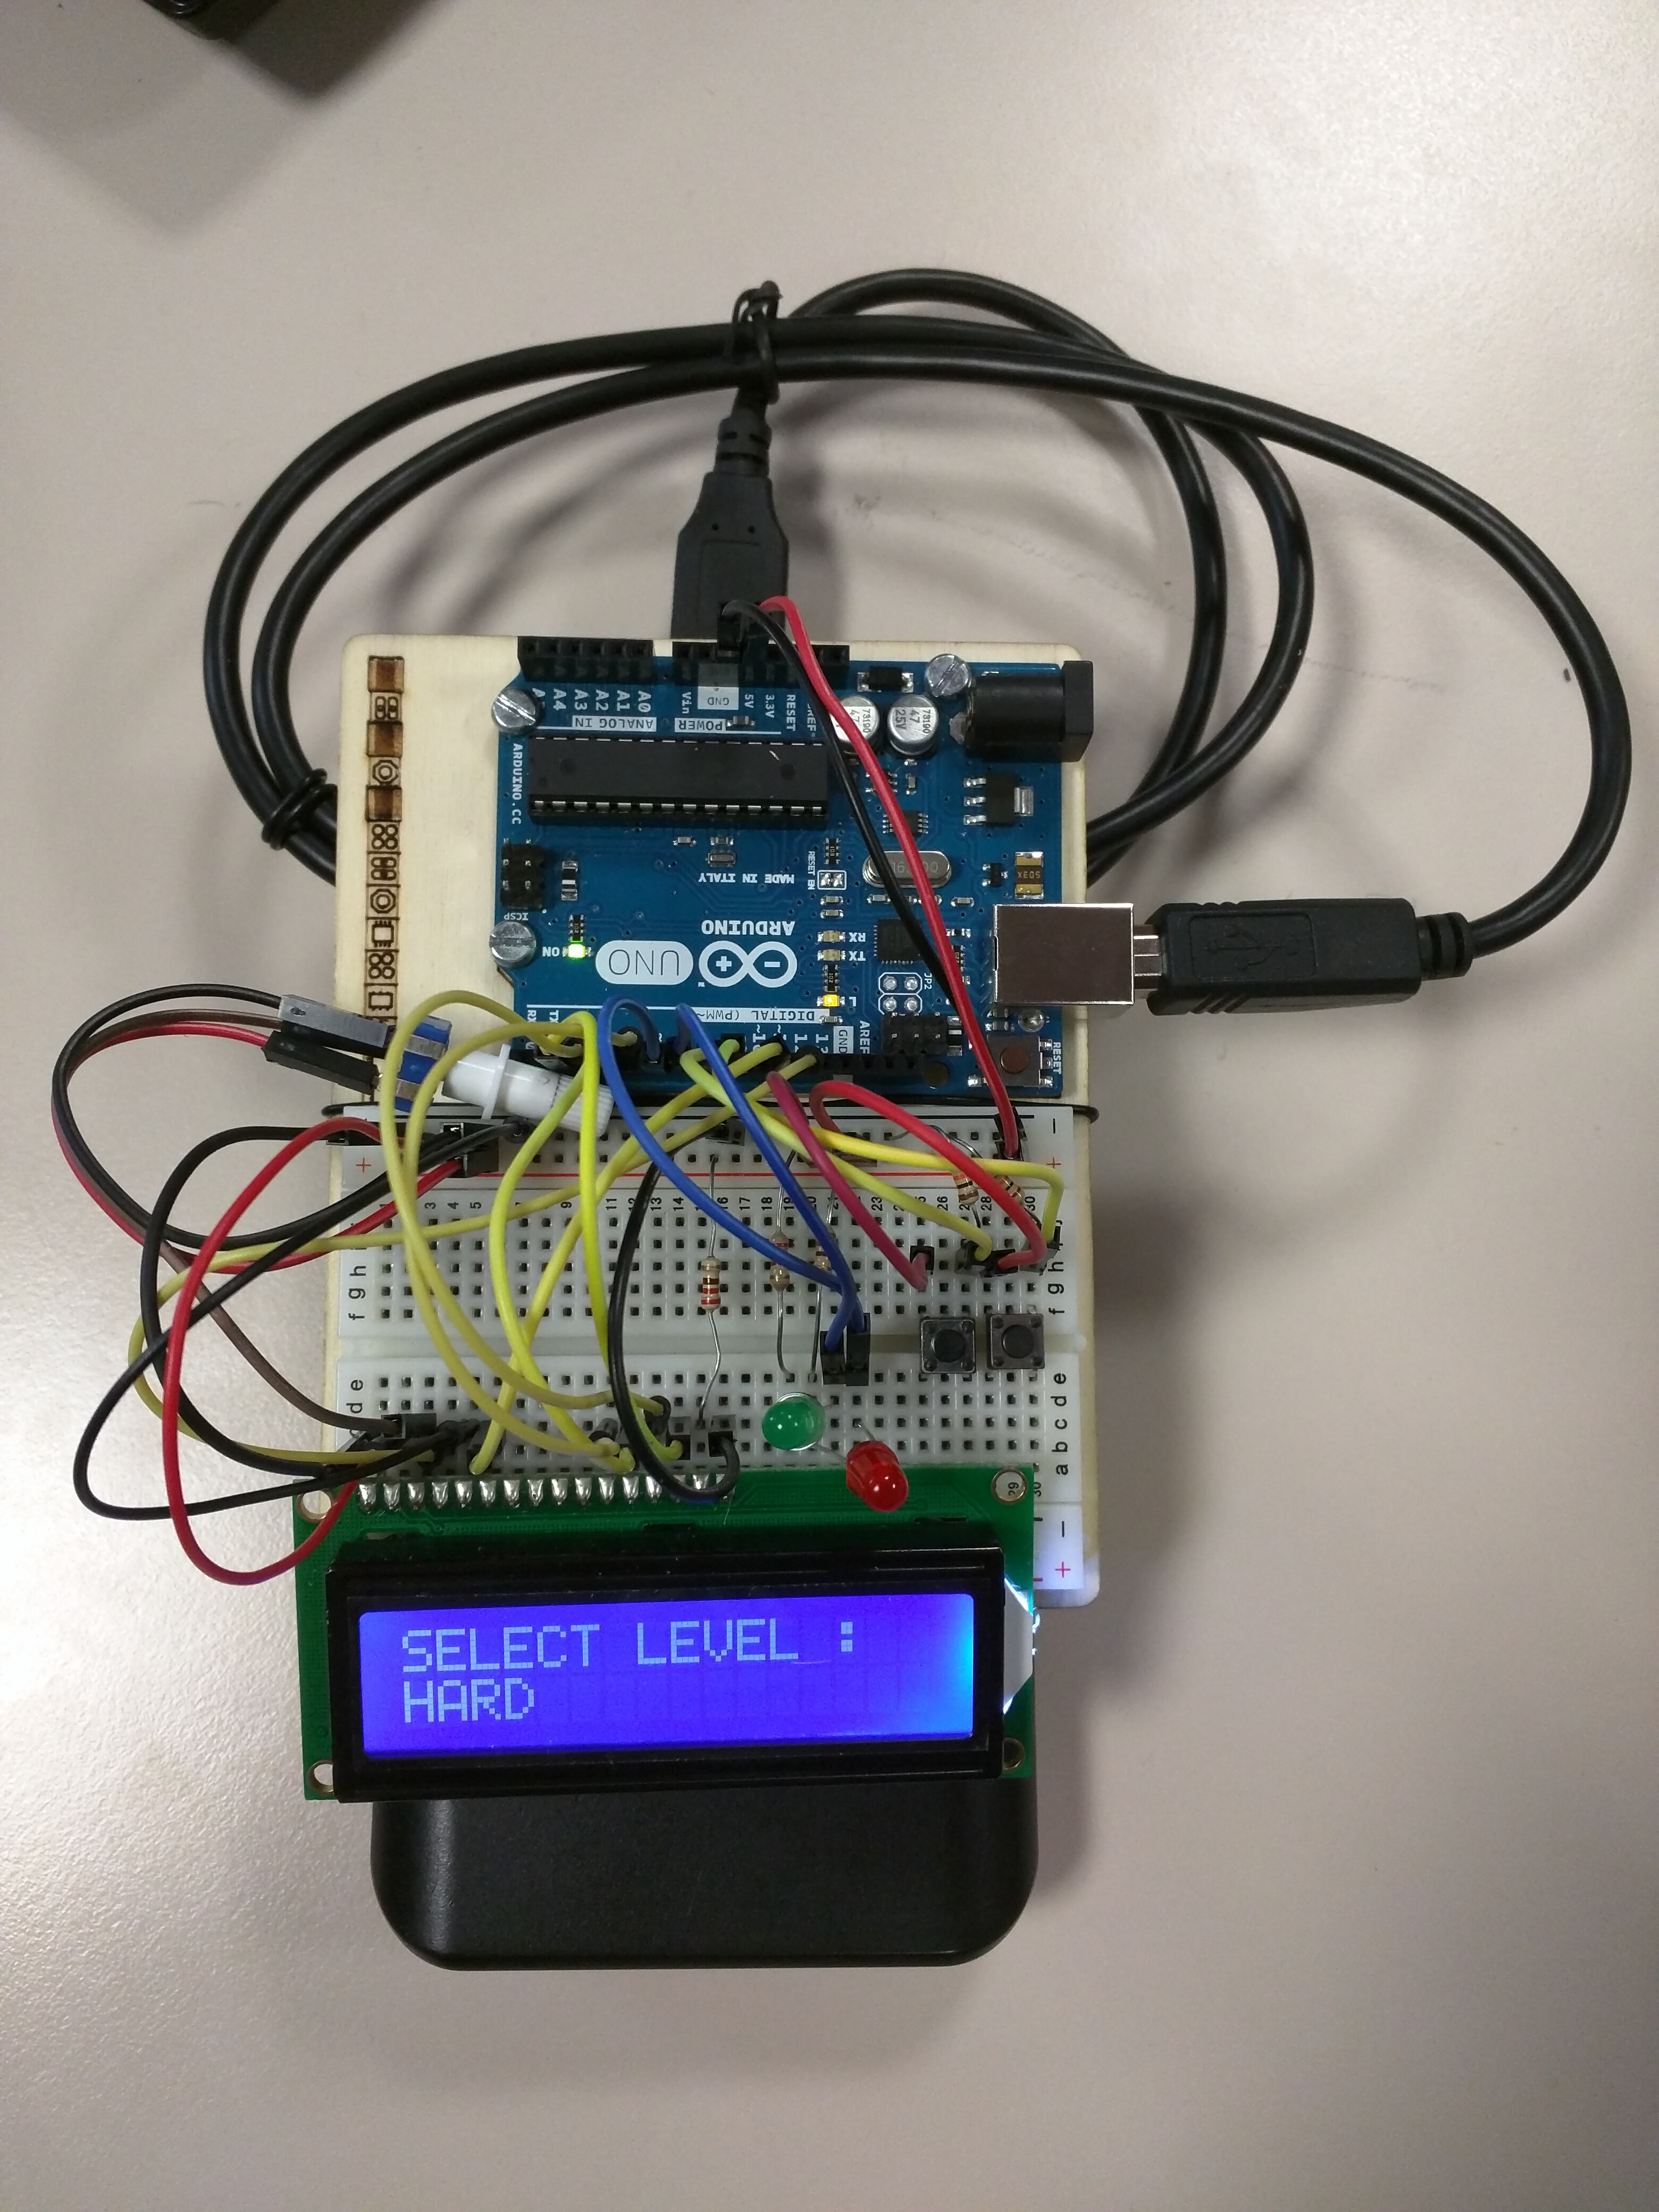
\includegraphics[height=18cm]{1.jpg}
        \caption{Montage final avec batterie pour pouvoir jouer partout}
\end{figure}

\begin{figure}[h]
	\centering
		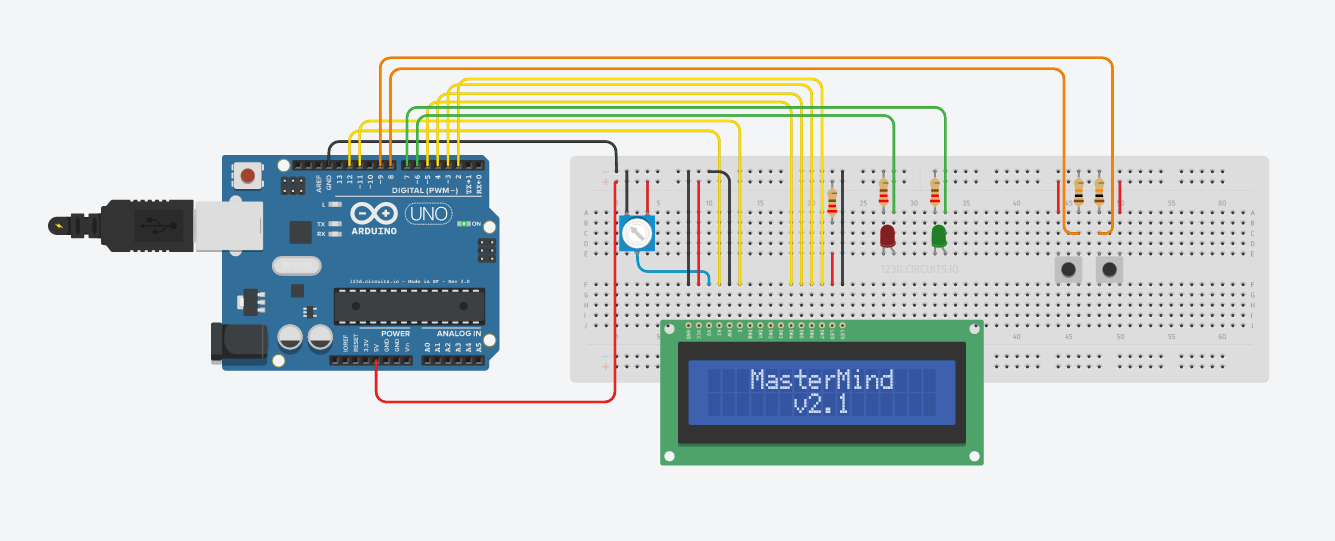
\includegraphics[width=\linewidth]{affichagefinal.png}
        \caption{Montage final du Projet Mastermind}
\end{figure}

\begin{figure}[h]
	\centering
      \subfloat[Début de partie]{\label{3}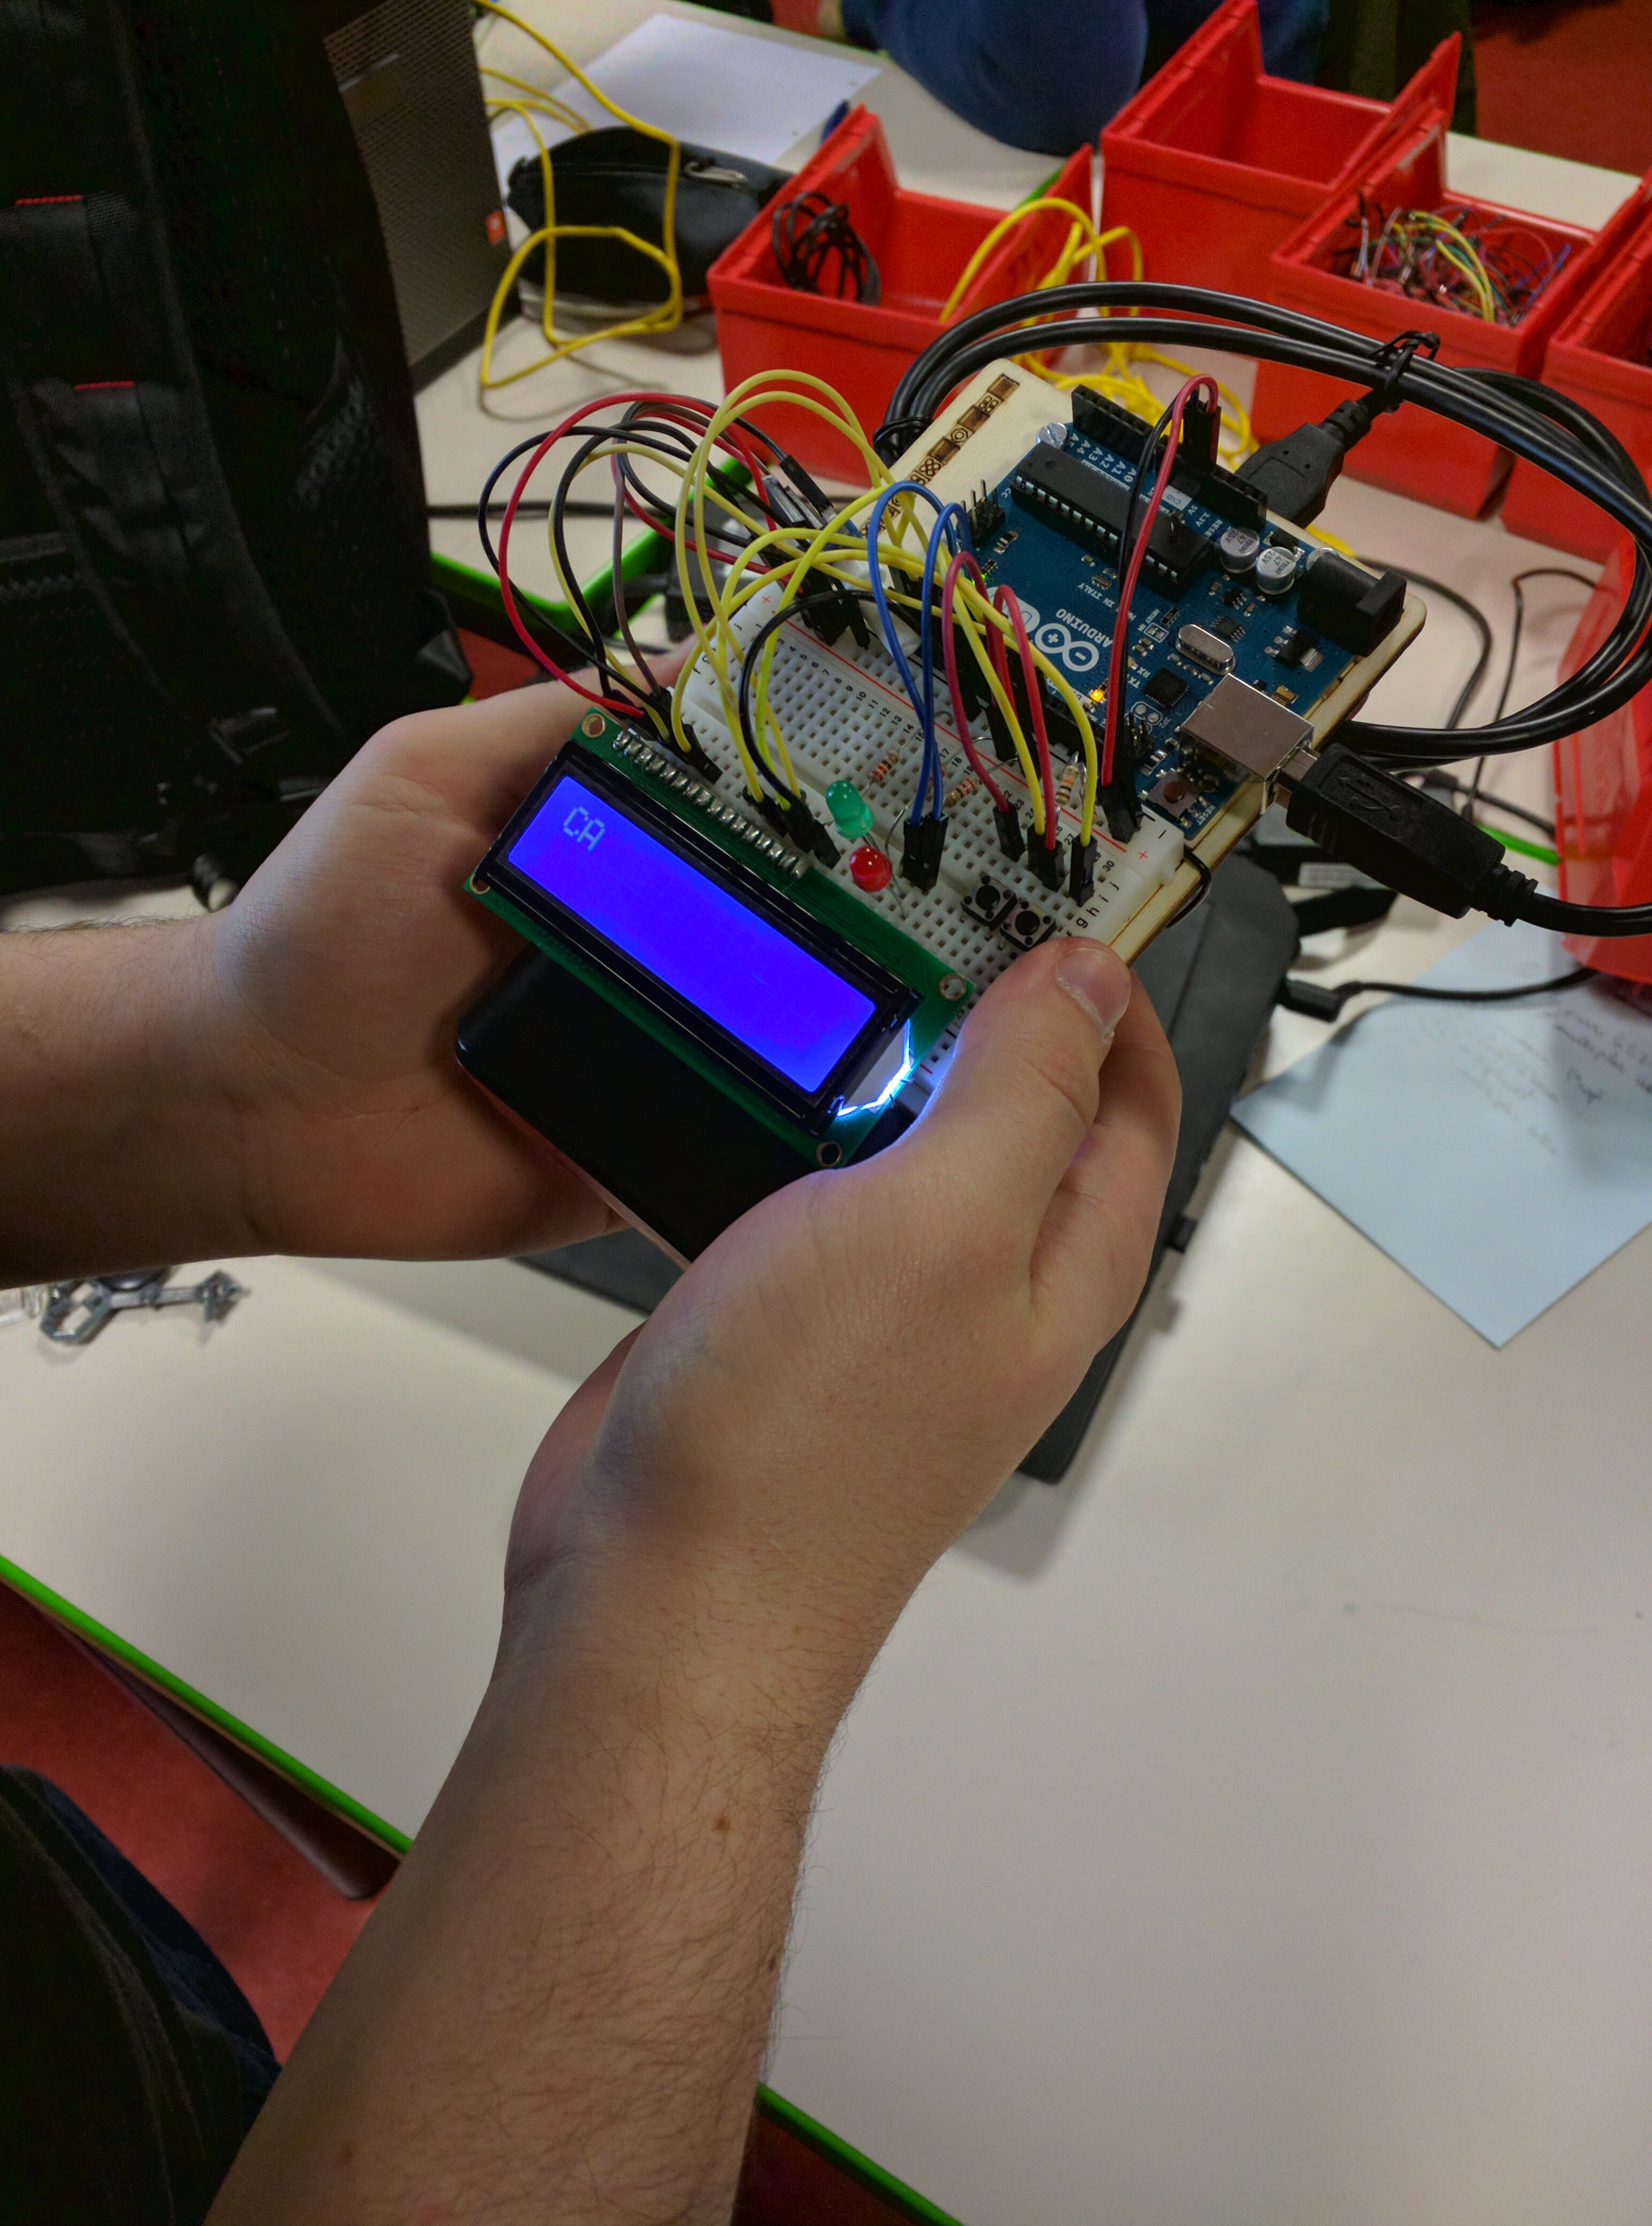
\includegraphics[width=8cm]{2.jpg}}
      \hspace{2mm}
      \subfloat[Partie de Mastermind]{\label{4}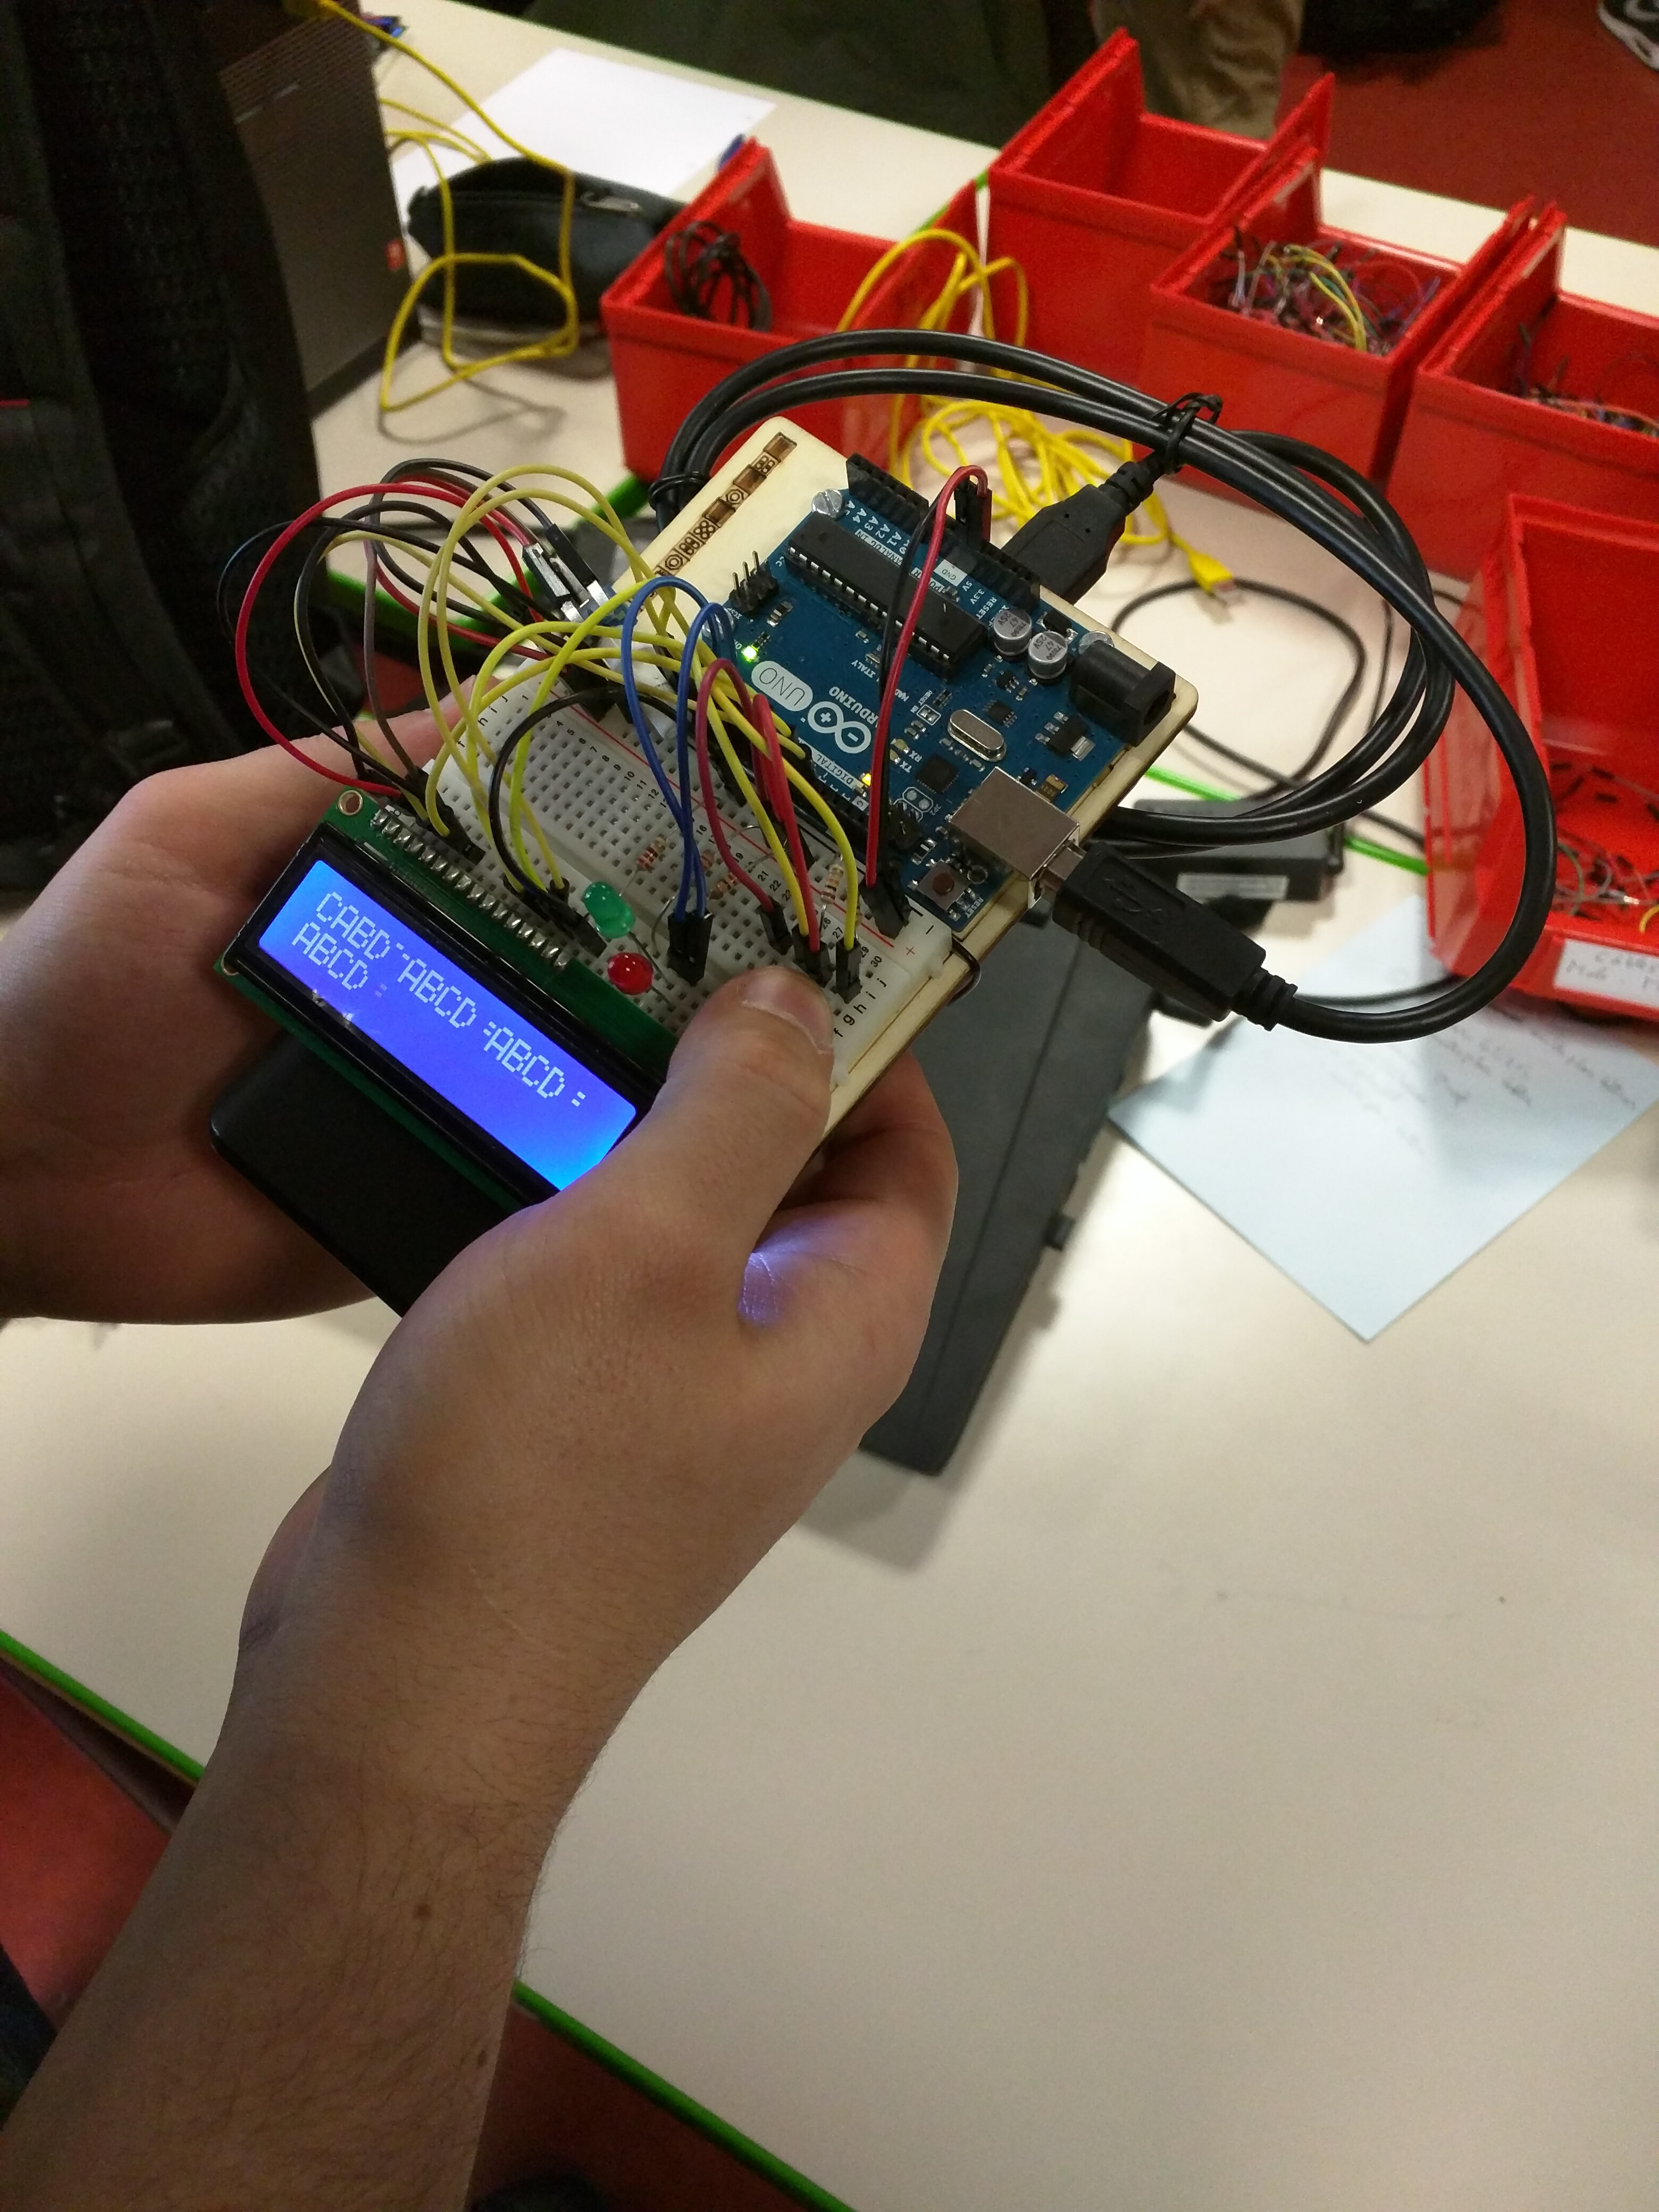
\includegraphics[width=8cm]{3.jpg}}
\end{figure}

\begin{figure}[h]
	\centering
		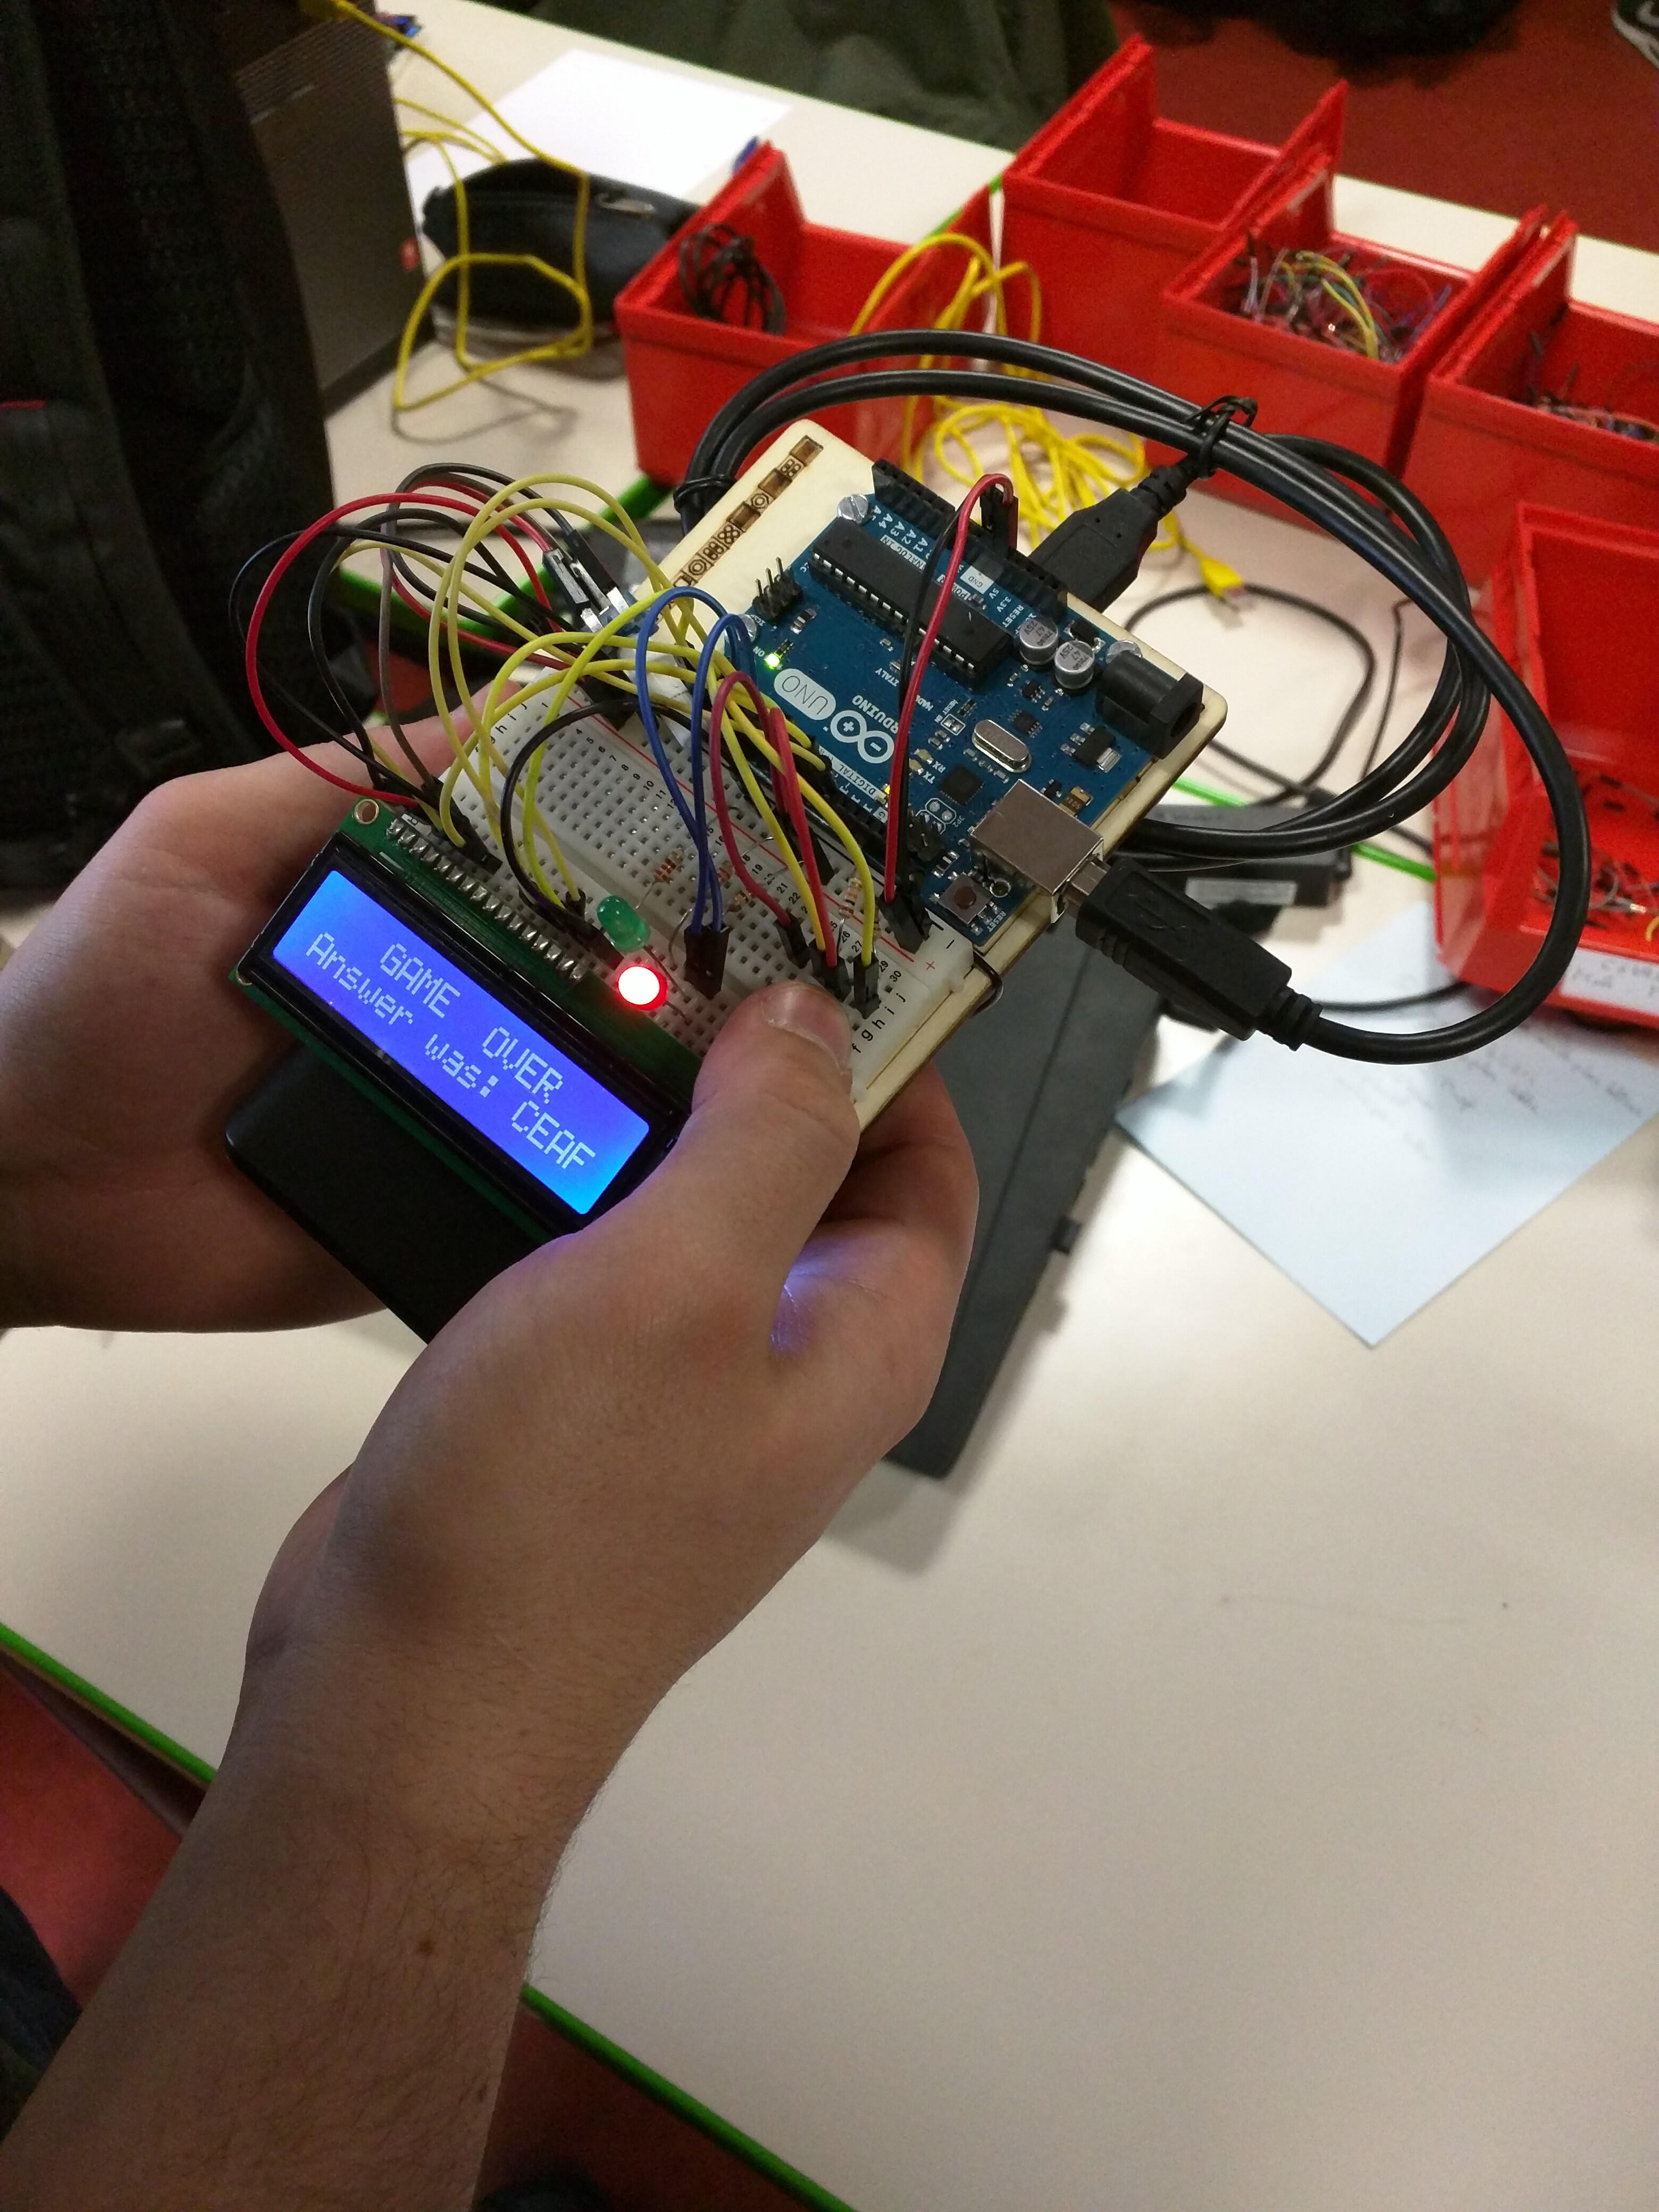
\includegraphics[width=18cm]{4.jpg}
        \caption{Fin de partie}
\end{figure}